% AcademiX - Presentación Entrega 3 (consolidada).
% Compilar con pdfLaTeX desde este directorio: latexmk -pdf main.tex
% Los bloques de cada integrante viven en <integrante>/NN-tema/frames.tex y se incluyen
% con \input; el preámbulo debe contener todo lo que esos bloques usan.
\documentclass[aspectratio=169,10pt]{beamer}

\usetheme{Boadilla}
\usepackage[utf8]{inputenc}
\usepackage[T1]{fontenc}
\usepackage[spanish,es-noshorthands]{babel}
\usepackage{graphicx}
\usepackage{tabularx}
\usepackage{booktabs}
\usepackage{xcolor}
\usepackage{tikz}
\usepackage{array}
\usepackage{pgfplots}

\usetikzlibrary{arrows.meta,positioning,fit,calc,shapes.geometric}
\pgfplotsset{compat=1.18}
\graphicspath{{dvillas28/img/}}

\definecolor{academixnavy}{HTML}{18324F}
\definecolor{academixblue}{HTML}{2563EB}
\definecolor{academixteal}{HTML}{0F766E}
\definecolor{academixamber}{HTML}{B7791F}
\definecolor{academixgreen}{HTML}{15803D}
\definecolor{academixred}{HTML}{B91C1C}
\definecolor{academixbg}{HTML}{F8FAFC}
\definecolor{academixsoftblue}{HTML}{EFF6FF}
\definecolor{academixsoftteal}{HTML}{F0FDFA}
\definecolor{academixsoftamber}{HTML}{FFFBEB}
\definecolor{academixline}{HTML}{CBD5E1}
\definecolor{academixslate}{HTML}{475569}
\definecolor{academixmuted}{HTML}{64748B}

\setbeamercolor{structure}{fg=academixnavy}
\setbeamercolor{frametitle}{fg=academixnavy,bg=academixbg}
\setbeamercolor{title}{fg=academixnavy}
\setbeamercolor{block title}{fg=white,bg=academixnavy}
\setbeamercolor{block body}{fg=black,bg=academixbg}
\setbeamercolor{alerted text}{fg=academixamber}
\setbeamertemplate{navigation symbols}{}
\setbeamertemplate{footline}[frame number]
\setbeamerfont{frametitle}{size=\large,series=\bfseries}
\setbeamerfont{title}{series=\bfseries}

\newcolumntype{Y}{>{\raggedright\arraybackslash}X}
\newcommand{\chip}[2]{\tikz[baseline=(n.base)]\node[rounded corners=2pt,fill=#1,inner xsep=5pt,inner ysep=2pt,text=white,font=\scriptsize\bfseries](n){#2};}
\newcommand{\softchip}[3]{\tikz[baseline=(n.base)]\node[rounded corners=2pt,draw=#1,fill=#2,inner xsep=5pt,inner ysep=2pt,text=#1,font=\scriptsize\bfseries](n){#3};}
\newcommand{\kpi}[3]{%
\begin{tikzpicture}
  \node[draw=#1,fill=#1!7,rounded corners=3pt,minimum width=0.28\textwidth,minimum height=1.15cm,align=center] {
    {\Large\bfseries\color{#1}#2}\\[-1pt]
    {\scriptsize #3}
  };
\end{tikzpicture}}

% Estilo común de los gráficos del tablero.
\pgfplotsset{academix/.style={
  width=\linewidth, height=5.6cm,
  font=\sffamily\scriptsize,
  axis lines=left, axis line style={academixslate},
  tick style={academixslate}, tick label style={academixslate},
  grid=major, grid style={academixline!60},
  legend style={draw=none,fill=none,font=\sffamily\scriptsize,legend columns=-1,
    at={(0.5,-0.14)},anchor=north,/tikz/every even column/.append style={column sep=6pt}},
  xmin=10.5, xmax=32.5,
  xtick={11,14,17,20,23,26,29,32}, xticklabels={11/10,14/10,17/10,20/10,23/10,26/10,29/10,1/11},
}}

\title[AcademiX]{AcademiX}
\subtitle{Entrega 3: desarrollo, métricas y plan hacia el MVP}
\author[Equipo Lock In]{Equipo Lock In}
\institute[IIC3143]{IIC3143 Desarrollo de Software}
\date{Noviembre 2026}

\begin{document}

\begin{frame}
  \titlepage
  \vspace{-0.25cm}
  \centering
  \softchip{academixnavy}{academixsoftblue}{Proceso}
  \softchip{academixteal}{academixsoftteal}{Calidad}
  \softchip{academixamber}{academixsoftamber}{CI/CD}
  \softchip{academixgreen}{green!8}{Métricas}
  \softchip{academixslate}{academixbg}{Plan}
\end{frame}

\begin{frame}{La respuesta primero}
\begin{columns}[T,onlytextwidth]
\begin{column}{0.48\textwidth}
\begin{block}{¿Alcanzamos?}
\small
\textbf{Sí}, el MVP comprometido: quedan 58 h de P0 y P1 en 3 semanas y el ritmo observado es de 97 h por semana.\\[0.15cm]
Material en archivos (P2, 21 h) queda condicionado al storage.
\end{block}
\centering
\kpi{academixgreen}{83\,\%}{386 de 465 h estimadas}
\end{column}
\begin{column}{0.48\textwidth}
\small
\textbf{Recorrido}
\begin{enumerate}
  \item Proceso: ciclo, tablero, prácticas y decisiones.
  \item Calidad: testing, cobertura y defectos.
  \item CI/CD: pipeline, SCA, SAST y revisión con IA.
  \item Métricas: burnup, CFD y tiempos.
  \item Plan: completo, pendiente y proyección.
  \item Demo.
\end{enumerate}
\end{column}
\end{columns}
\end{frame}

% 1. Proceso de desarrollo
% E3-04/05/06: ciclo de desarrollo, PR y merges, prácticas y beneficios.
% Fuente: gh pr list (merged), rulesets de dev y main, git-flow.md. Corte 01/11.
% Capturas de la PR #86 en img/, tomadas por dvillas28 el 01/11.

\begin{frame}{Ciclo de desarrollo: de la tarjeta a producción}
\centering
\begin{tikzpicture}[
  stage/.style={draw=academixnavy,fill=academixsoftblue,rounded corners=3pt,font=\scriptsize\bfseries,
    text=academixnavy,minimum height=0.95cm,text width=1.45cm,inner xsep=2pt,align=center},
  gate/.style={draw=academixamber,fill=academixsoftamber,rounded corners=3pt,font=\scriptsize\bfseries,
    text=academixamber,minimum height=0.95cm,text width=1.45cm,inner xsep=2pt,align=center},
  note/.style={font=\tiny,text=academixslate,text width=1.65cm,align=center},
  arr/.style={-{Stealth[length=2mm]},academixslate,thick},
  node distance=0.3cm]
\node[stage] (a) {Issue o spec};
\node[stage,right=of a] (b) {Rama\\\texttt{tipo/nombre}};
\node[stage,right=of b] (c) {PR a \texttt{dev}};
\node[gate,right=of c] (d) {CI result + bot IA};
\node[stage,right=of d] (e) {Squash a \texttt{dev}};
\node[stage,right=of e] (f) {Merge a \texttt{main}};
\node[gate,right=of f] (g) {Release + Render};
\foreach \x/\y in {a/b,b/c,c/d,d/e,e/f,f/g} \draw[arr] (\x) -- (\y);
\node[note,below=0.15cm of a] {Tarjeta en el tablero con horas estimadas};
\node[note,below=0.15cm of b] {In progress al crear la rama};
\node[note,below=0.15cm of c] {Revisión de un par: no obligatoria};
\node[note,below=0.15cm of d] {Sin CI verde no hay merge};
\node[note,below=0.15cm of e] {Tag \texttt{vX.Y.Z-dev.N}};
\node[note,below=0.15cm of f] {Merge commit, sin squash};
\node[note,below=0.15cm of g] {Deploy tras pasar CI};
\end{tikzpicture}
\vspace{0.45cm}

\begin{columns}[T,onlytextwidth]
\begin{column}{0.31\textwidth}\centering\kpi{academixnavy}{68}{PR integradas desde el 11/10}\end{column}
\begin{column}{0.31\textwidth}\centering\kpi{academixteal}{54 / 13}{a \texttt{dev} / a \texttt{main}}\end{column}
\begin{column}{0.31\textwidth}\centering\kpi{academixamber}{23 de 68}{con revisión de un par}\end{column}
\end{columns}
\vspace{0.2cm}
\scriptsize Reglas en GitHub: \texttt{dev} solo acepta squash; \texttt{main} solo merge commit. Ambas exigen el check \texttt{CI result} y bloquean force push y borrado.
\end{frame}

\begin{frame}{Una PR real: \#86, cursos y roles}
\begin{columns}[T,onlytextwidth]
\begin{column}{0.6\textwidth}
\centering

\includegraphics[height=6.6cm]{pr-86-full}
\end{column}
\begin{column}{0.37\textwidth}
\small
\begin{itemize}
  \item Título en conventional commits: define la versión del release.
  \item De \texttt{feat/cursos-roles-backend} a \texttt{dev}.
  \item Enlaza el spec y la evidencia de validación, y cierra 4 issues del backlog.
  \item 12 checks en verde: CI, SonarQube y Trivy.
  \item \texttt{CI result} habilita el merge.
\end{itemize}
\end{column}
\end{columns}
\end{frame}

\begin{frame}{Prácticas que usamos y qué nos dieron}
\small
\begin{tabularx}{\textwidth}{>{\raggedright\arraybackslash}p{3.1cm}YY}
\toprule
\textbf{Práctica} & \textbf{Evidencia} & \textbf{Beneficio observado} \\
\midrule
Spec Kit antes de codificar & \texttt{specs/} por funcionalidad, con CU y RF & El alcance de cada PR está escrito antes del código \\
ADR & 22 decisiones en \texttt{docs/adr/} & El cambio de Railway a Render quedó trazado con contexto y costos \\
Conventional commits & 67 tags y releases automáticos & Cada versión en Render se identifica en \texttt{/health} \\
CI como gate & \texttt{CI result} obligatorio en \texttt{dev} y \texttt{main} & 35 ejecuciones fallidas en PR detuvieron el merge hasta corregir \\
Tests de aislamiento & UC y UTFSM, RLS y E2E de tenant & El aislamiento se prueba en cada PR, no solo antes de la demo \\
Tablero con horas & Backlog GitHub Projects & Proyección del pendiente en horas \\
\bottomrule
\end{tabularx}
\vspace{0.2cm}

\scriptsize Pendiente de mejora: la revisión de un par no es obligatoria (34\,\% de las PR la tuvieron) y la etiqueta \texttt{bug} no se usa.
\end{frame}

% E3-12, E3-13: cuándo una tarjeta avanza de estado y cuándo está Done.
% Fuentes: docs/guides/board-metrics.md; conteo por estado del snapshot del 01/11.

\begin{frame}{Cómo se mueve una tarjeta}
\centering
\begin{tikzpicture}[
  font=\sffamily\small,
  st/.style={rounded corners=5pt,minimum width=2.5cm,minimum height=1.25cm,align=center,very thick},
  rule/.style={font=\sffamily\scriptsize,text width=3.1cm,align=center,text=academixslate,anchor=south},
  arr/.style={-{Latex[length=2.5mm]},draw=academixnavy,very thick}
]
\node[st,draw=academixslate,fill=academixbg] (d) at (0,0) {\textbf{Draft}\\{\scriptsize idea en el backlog}};
\node[st,draw=academixblue,fill=academixsoftblue] (t) at (4,0) {\textbf{Todo}\\{\Large\bfseries 27}};
\node[st,draw=academixamber,fill=academixsoftamber] (p) at (8,0) {\textbf{In progress}\\{\Large\bfseries 0}};
\node[st,draw=academixgreen,fill=green!8] (o) at (12,0) {\textbf{Done}\\{\Large\bfseries 96}};
\draw[arr] (d) -- (t);
\node[rule] at (2,0.85) {Se convierte en issue al iniciar su semana};
\draw[arr] (t) -- (p);
\node[rule] at (6,0.85) {Alguien empieza\\a trabajarla};
\draw[arr] (p) -- (o);
\node[rule] at (10,0.85) {Su PR está en \texttt{dev} y tiene \texttt{Real (h)}};
\node[font=\sffamily\scriptsize,text=academixmuted] at (6,-1.0) {tarjetas por estado al 01/11};
\end{tikzpicture}
\vspace{0.3cm}

\begin{columns}[T,onlytextwidth]
\begin{column}{0.48\textwidth}
\begin{block}{Cada tarjeta lleva}
\scriptsize
Semana, tipo, área, prioridad, responsable, horas estimadas y, al cerrar, horas reales. Las PR se vinculan a su issue con \texttt{Closes \#N}.
\end{block}
\end{column}
\begin{column}{0.48\textwidth}
\begin{block}{Snapshot diario}
\scriptsize
Un workflow exporta el tablero cada noche a la rama \texttt{metrics}. Con esos snapshots salen el burnup, el CFD y los tiempos de las métricas.
\end{block}
\end{column}
\end{columns}
\end{frame}

% E3-07: prácticas abandonadas o no cumplidas.
% Fuentes: conciliacion-tablero-e3.md (bloques C, D y F), ADR de Render.

\begin{frame}{Prácticas abandonadas o no cumplidas}
\small
\begin{tabularx}{\textwidth}{>{\raggedright\arraybackslash}p{3.3cm}YY}
\toprule
\textbf{Práctica} & \textbf{Qué pasó} & \textbf{Qué hacemos ahora} \\
\midrule
Reporte de seguridad con Semgrep (\#57) & SonarQube y Trivy ya cubrían el análisis en cada PR. & Cerrada como \emph{not planned}. \\
Convertir drafts en issue al iniciar la semana & No se aplicó desde la semana 4: las PR no podían cerrar sus tarjetas. & Todas las issues drafts se convirtieron en issues. \\
Registrar \texttt{Real (h)} al cerrar & Al 30/10, 77 de 87 tarjetas Done sin horas reales. & Completadas a posteriori: al 01/11, 68 de 96 tienen horas. \\
Railway como plataforma & Despliegues pausados tras su incidente de seguridad del 21/10. & Render, con ADR y tarjetas \#175–\#177. \\
Backup y PITR en Railway & Teníamos pocos datos en Railway; asumimos el costo de no respaldar. & Levantamos todo desde 0 en Render. \\
\bottomrule
\end{tabularx}
\vspace{0.3cm}

\centering
\large\textbf{\color{academixnavy}Las reglas del tablero existían; faltó revisarlas cada semana.}
\end{frame}

% E3-08, E3-29/30: migración de Railway a Render.
% Fuentes: docs/adr/deploy-on-render.md, issues #175–#178.

\begin{frame}{Decisión: de Railway a Render (22/10)}
\begin{columns}[T,onlytextwidth]
\begin{column}{0.48\textwidth}
\begin{block}{Contexto}
\small El 21/10 Railway sufrió un grave incidente de seguridad: un atacante accedió a los sistemas que guardan las variables de entorno de sus clientes. Como medida, Railway pausó los despliegues.
\end{block}
\begin{block}{Decisión}
\small
\begin{itemize}
  \item Blueprint \texttt{render.yaml}: backend, frontend y PostgreSQL 17.
  \item Deploy de \texttt{main} solo si pasan todos los checks.
  \item Plan free: migraciones al arrancar.
\end{itemize}
\end{block}
\end{column}
\begin{column}{0.48\textwidth}
\begin{block}{Qué no cambió}
\small
\begin{itemize}
  \item Dockerfiles, CI, Trivy, Sonar y Release.
  \item RLS, rol runtime sin bypass y retiro de secretos.
\end{itemize}
\end{block}
\begin{block}{Costos aceptados}
\small
\begin{itemize}
  \item Arranque en frío de $\sim$1 min tras 15 min sin tráfico.
  \item 750 h/mes compartidas entre servicios.
  \item La base expira a los 30 días, sin respaldos.
\end{itemize}
\end{block}
\end{column}
\end{columns}
\end{frame}


% 2. Calidad y testing
% E3-17 a E3-19: estrategia de testing y flujos de usuario probados.
% Fuente: logs de la auditoría SonarQube del 01/11 (conteo de tests de BE y FE),
% e2e.yml (run 41338806749), docs/testing (catálogo E2E y corrida F7 del 31/10),
% backend/test/integration y frontend/test.

\begin{frame}{Estrategia de testing}
\begin{columns}[T,onlytextwidth]
\begin{column}{0.5\textwidth}
\centering
\begin{tikzpicture}[lvl/.style={align=center,font=\scriptsize,text=white}]
\fill[academixnavy] (-3.0,0) -- (3.0,0) -- (2.2,1.2) -- (-2.2,1.2) -- cycle;
\fill[academixteal] (-2.2,1.2) -- (2.2,1.2) -- (1.4,2.4) -- (-1.4,2.4) -- cycle;
\fill[academixamber] (-1.4,2.4) -- (1.4,2.4) -- (0.55,3.5) -- (-0.55,3.5) -- cycle;
\node[lvl] at (0,0.6) {\textbf{Unitarias y DOM}\\350 frontend};
\node[lvl] at (0,1.8) {\textbf{Integración}\\207 backend, PostgreSQL real};
\node[lvl] at (0,2.85) {\textbf{E2E}\\248 casos};
\end{tikzpicture}
\end{column}
\begin{column}{0.48\textwidth}
\scriptsize
\begin{itemize}
  \item \textbf{Backend:} \texttt{node:test} contra PostgreSQL con RLS y el rol de runtime real; HTTP, roles y aislamiento UC/UTFSM.
  \item \textbf{Frontend:} \texttt{node:test} con DOM simulado; componentes, sesión y cliente de API.
  \item \textbf{E2E:} Playwright con API y base reales; 20 specs, 5 de seguridad (tenant, RBAC, auth, admin, auditoría). 13 min en CI.
\end{itemize}
\textbf{Por qué así:} lo más importante es asegurar que una institución no pueda acceder a los datos de otra y que las notas no sean visibles antes de publicarlas. Por eso realizamos pruebas con una base de datos real, además de las pruebas con mocks.
\end{column}
\end{columns}
\end{frame}

\begin{frame}{Qué probamos: flujos de usuario}
\scriptsize
\renewcommand{\arraystretch}{1.15}
\begin{tabularx}{\textwidth}{>{\raggedright\arraybackslash}p{3.6cm}rrrY}
\toprule
\textbf{Flujo} & \textbf{E2E} & \textbf{Integ. BE} & \textbf{Unit. FE} & \textbf{Qué asegura} \\
\midrule
Entrar a mi institución & 44 & 7 & 5 & Login global, sesión en memoria y una cuenta de UC que no ve UTFSM \\
Docente arma su curso & 38 & 8 & 6 & Creación atómica, secciones y asignar, revocar y reactivar roles \\
Docente publica material & 16 & 7 & 9 & Módulos ordenados, visibilidad y Markdown seguro \\
Docente crea y publica un quiz & 18 & 7 & 11 & Borrador validado, publicación irreversible y pauta protegida \\
Estudiante rinde el quiz & 32 & 7 & 10 & Guardar respuestas, envío atómico con autocorrección y cancelación \\
Notas: ponderar, publicar y consultar & 42 & 12 & 11 & Cálculo decimal, pesos congelados, nota visible solo al publicar y auditoría \\
\midrule
\textbf{Total} & \textbf{248} & \textbf{66} & \textbf{55} & \\
\bottomrule
\end{tabularx}
\vspace{0.2cm}

E2E: fichas del catálogo; los totales suman además permisos (13), administración (11), red (13), accesibilidad (8), operación (9) y catálogo de API (4). Integración y unitarias: archivos de test; el resto es operación, seed y componentes compartidos.\\[0.15cm]
\centering
\softchip{academixgreen}{green!8}{Corrida completa del 31/10: 248 fichas, 512 ejecuciones en Chromium, Firefox y WebKit, 0 fallos}
\end{frame}


% 3. CI/CD
% E3-22: pipeline y etapas; requisitos de la pauta: SCA, SAST y code review con IA.
% Fuente: .github/workflows/*.yml; ejecuciones desde el 11/10; auditorías manuales
% del 01/11 (runs 41338835122 Trivy y 41338849373 SonarQube); capturas en img/.

\begin{frame}{Pipeline de CI/CD}
\centering
\begin{tikzpicture}[
  job/.style={draw=academixnavy,fill=academixsoftblue,rounded corners=3pt,font=\scriptsize,
    text=academixnavy,minimum height=0.62cm,text width=2.7cm,align=center},
  sec/.style={draw=academixamber,fill=academixsoftamber,rounded corners=3pt,font=\scriptsize,
    text=academixamber,minimum height=0.62cm,text width=2.7cm,align=center},
  okjob/.style={draw=academixgreen,fill=green!6,rounded corners=3pt,font=\scriptsize\bfseries,
    text=academixgreen,minimum height=0.62cm,text width=2.2cm,align=center},
  lane/.style={font=\scriptsize\bfseries,text=academixslate,anchor=east},
  arr/.style={-{Stealth[length=1.8mm]},academixslate}]
% PR
\node[job] (doc) at (0,0) {Largo de documentos};
\node[job] (api) at (0,-0.75) {OpenAPI y cliente generado};
\node[job] (lint) at (0,-1.5) {Lint + test / build\\[-1pt]\tiny por app, solo si cambió};
\node[sec] (dock) at (3.2,0) {Docker build + Trivy\\[-1pt]\tiny imagen y dependencias};
\node[job] (cov) at (3.2,-0.75) {Integración PostgreSQL + cobertura};
\node[sec] (sonar) at (3.2,-1.5) {SonarQube\\[-1pt]\tiny quality gate};
\node[okjob] (ci) at (6.3,-0.75) {CI result\\[-1pt]\tiny check obligatorio};
\node[sec] (bot) at (3.2,-2.55) {Bot reviewer IA\\[-1pt]\tiny comenta el diff};
\node[job] (e2e) at (0,-2.55) {E2E Playwright\\[-1pt]\tiny 20 specs};
\draw[arr] (cov) -- (sonar);
\node[draw=academixgreen,dashed,rounded corners=4pt,inner sep=4pt,fit=(doc)(lint)(dock)(sonar)] (gate) {};
\draw[arr] (gate.east |- ci.west) -- (ci.west);
\node[font=\tiny,text=academixslate,anchor=west] at (bot.east) {corren en la PR, no bloquean};
% merge
\node[okjob] (dev) at (9.0,0) {Squash a \texttt{dev}};
\node[job,text width=2.2cm] (tag) at (9.0,-0.75) {Tag \texttt{-dev.N}};
\node[okjob] (main) at (9.0,-1.5) {Merge a \texttt{main}};
\node[job,text width=2.2cm] (rel) at (11.6,-1.5) {Release \texttt{vX.Y.Z}};
\node[sec,text width=2.2cm] (render) at (11.6,-0.75) {Deploy Render};
\draw[arr] (ci.east) -- (dev.west);
\draw[arr] (dev) -- (tag);
\draw[arr] (tag) -- (main);
\draw[arr] (main) -- (rel);
\draw[arr] (main.north east) -- (render.south west);
\node[font=\tiny,text=academixslate,align=center] at (11.6,0) {Auto-deploy:\\after CI checks pass};
\node[lane] at (-1.6,0.55) {PR};
\node[lane,anchor=west] at (8.0,0.55) {Integración};
\end{tikzpicture}
\vspace{0.3cm}

\begin{columns}[T,onlytextwidth]
\begin{column}{0.23\textwidth}\centering\kpi{academixnavy}{137 / 181}{CI exitosas desde 11/10}\end{column}
\begin{column}{0.23\textwidth}\centering\kpi{academixgreen}{67 / 67}{releases y tags}\end{column}
\begin{column}{0.23\textwidth}\centering\kpi{academixteal}{8 / 9}{E2E exitosas}\end{column}
\begin{column}{0.23\textwidth}\centering\kpi{academixamber}{16 / 18}{revisiones del bot}\end{column}
\end{columns}
\vspace{0.1cm}
\centering\scriptsize Las 36 ejecuciones fallidas de CI son casi todas de PR (35): el gate cumplió su función. E2E corre en PR, pero aún no es check obligatorio.
\end{frame}

\begin{frame}{Seguridad y calidad: SCA, SAST y revisión con IA}
\begin{columns}[T,onlytextwidth]
\begin{column}{0.32\textwidth}
\begin{block}{SCA: Trivy}
\scriptsize
\textbf{En CI:} \texttt{fs} e imagen Docker; falla con HIGH o CRITICAL con corrección.\\[0.15cm]
\textbf{Auditoría 01/11}, repo completo:
\begin{itemize}
  \item 0 CRITICAL, 0 HIGH.
  \item 3 MEDIUM en el backend: \texttt{glob}, \texttt{minimatch} y \texttt{qs}, todas con versión corregida.
\end{itemize}
\end{block}
\end{column}
\begin{column}{0.32\textwidth}
\begin{block}{SAST: SonarQube}
\scriptsize
\textbf{En CI:} quality gate que bloquea la PR.\\[0.15cm]
\textbf{Auditoría 01/11}, 9\,465 líneas:
\begin{itemize}
  \item Quality gate \textbf{OK}; cobertura 94,1\,\%; duplicación 0,0\,\%.
  \item 11 issues: 1 bug crítico (\texttt{sort} sin comparador en el libro de notas) y 10 code smells, 8 de ellos \texttt{tabIndex}.
\end{itemize}
\end{block}
\end{column}
\begin{column}{0.32\textwidth}
\begin{block}{Code review con IA}
\scriptsize
\textbf{Bot propio:} GitHub Actions + Gemini; lee el diff de cada PR a \texttt{dev} o \texttt{main} y comenta.\\[0.15cm]
Criterios del dominio: aislamiento, roles, notas y tests (ADR \texttt{define-bot-pr-reviewer}).
\begin{itemize}
  \item No bloquea: evita el riesgo R-16 de frenar el flujo.
  \item Pendiente: ajustar falsos positivos (\#173).
\end{itemize}
\end{block}
\end{column}
\end{columns}
\vspace{0.2cm}
\centering
\softchip{academixamber}{academixsoftamber}{El bug crítico y la actualización de dependencias se resuelven esta semana}
\end{frame}

\begin{frame}{Evidencia: auditorías del 01/11 sobre \texttt{main}}
\begin{columns}[T,onlytextwidth]
\begin{column}{0.36\textwidth}
\centering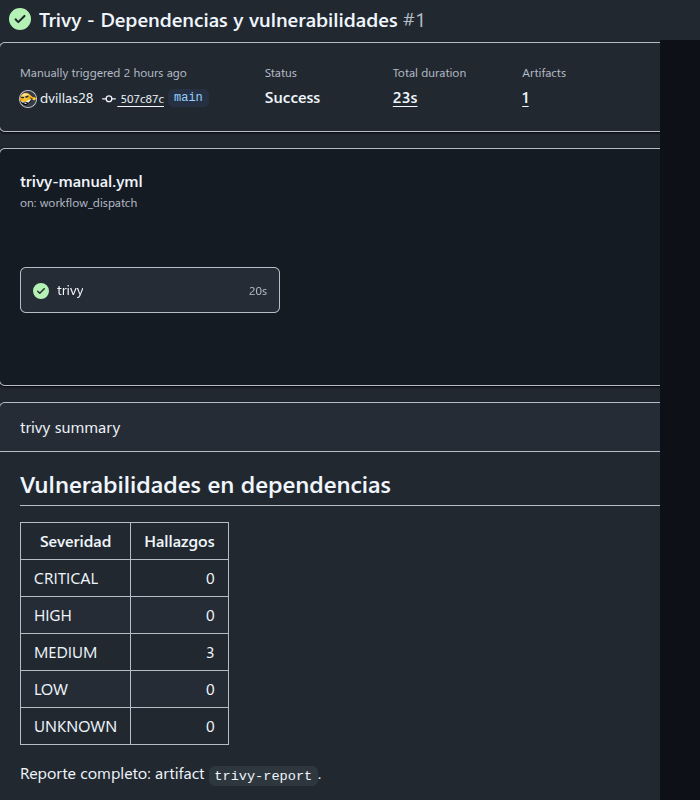
\includegraphics[width=\linewidth]{trivy-manual}
\end{column}
\begin{column}{0.36\textwidth}
\centering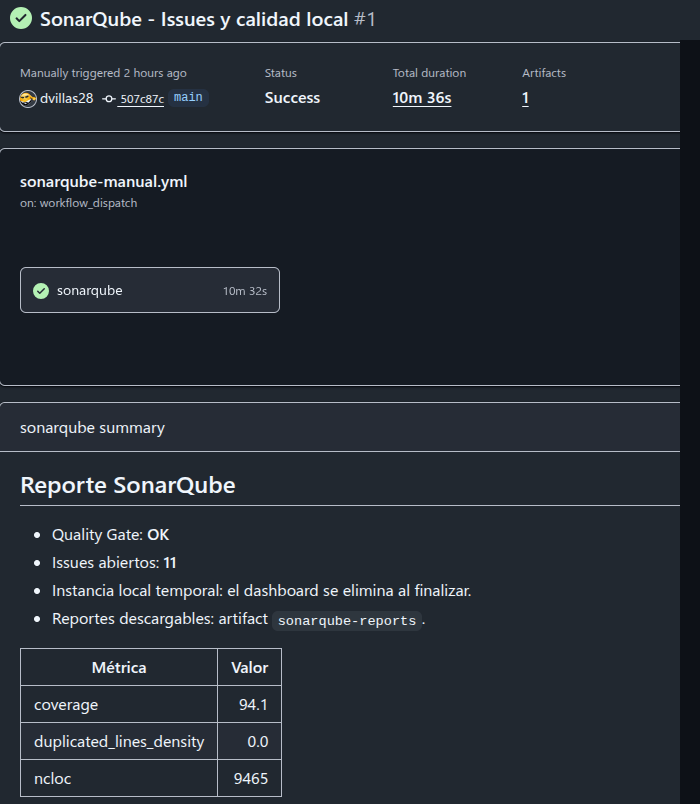
\includegraphics[width=\linewidth]{sonarqube-manual}
\end{column}
\begin{column}{0.24\textwidth}
\scriptsize
\textbf{Trivy (SCA)}\\
0 críticas y 0 altas. Las 3 medias tienen versión corregida.\\[0.25cm]
\textbf{SonarQube (SAST)}\\
Quality gate OK, cobertura 94,1\,\% y 0\,\% de duplicación en 9\,465 líneas.\\[0.25cm]
\textbf{Cómo se usan}\\
Se lanzan a pedido desde Actions y dejan el reporte como artifact. Los gates de cada PR siguen activos en CI.
\end{column}
\end{columns}
\end{frame}


% 4. Métricas
% E3-24: métricas del tablero. Datos: snapshots diarios de la rama metrics
% (11/10 a 01/11) procesados con scripts/board-metrics.mjs --csv. El 01/11 se
% volvió a tomar tras cargar las horas reales.
% Eje x: día de octubre; 32 = 01/11. El snapshot del 31/10 ya incluye la conciliación del 30/10.

\begin{frame}{Burnup: horas estimadas}
\begin{columns}[T,onlytextwidth]
\begin{column}{0.66\textwidth}
\begin{tikzpicture}
\begin{axis}[academix, ymin=0, ymax=520, ylabel={horas}]
\addplot[academixslate,thick,dashed,const plot] coordinates {
  (11,457) (25,457) (26,461) (30,461) (31,464) (32,465)};
\addlegendentry{alcance}
\addplot[academixnavy,very thick,const plot,mark=*,mark size=1pt] coordinates {
  (11,25) (12,25) (13,25) (14,25) (15,25) (16,29) (17,26) (18,26) (19,26) (20,28)
  (21,179) (22,185) (23,185) (24,185) (25,185) (26,207) (27,255) (28,255) (29,255) (30,255)};
\addlegendentry{terminado}
\addplot[academixamber,very thick,const plot,mark=*,mark size=1.5pt] coordinates {(30,255) (31,357) (32,386)};
\addlegendentry{tras conciliación}
\node[font=\sffamily\tiny,academixnavy,anchor=west,align=left] at (axis cs:21.4,100) {21/10: +151 h\\en un día};
\node[font=\sffamily\tiny,academixamber,anchor=east,align=right] at (axis cs:30.7,330) {31/10: +102 h\\ya integradas};
\end{axis}
\end{tikzpicture}
\end{column}
\begin{column}{0.31\textwidth}
\vspace{0.1cm}
\kpi{academixnavy}{83\,\%}{386 de 465 h}\\[0.2cm]
\kpi{academixteal}{78\,\%}{96 de 123 tarjetas}\\[0.2cm]
\scriptsize Los saltos del 21/10 y del 31/10 corresponden a actualizaciones del tablero por lotes.
\end{column}
\end{columns}
\end{frame}

\begin{frame}{Flujo acumulado (CFD)}
\centering
\begin{tikzpicture}
\begin{axis}[academix, width=0.85\linewidth, height=6cm, ymin=0, ymax=130, ylabel={tarjetas}, stack plots=y,
  area style, reverse legend]
\addplot[fill=academixgreen!35,draw=academixgreen] coordinates {
  (11,11) (12,11) (13,11) (14,11) (15,11) (16,12) (17,11) (18,11) (19,11) (20,12)
  (21,49) (22,50) (23,50) (24,50) (25,50) (26,55) (27,64) (28,64) (29,64) (30,64) (31,87) (32,96)} \closedcycle;
\addlegendentry{Done}
\addplot[fill=academixamber!45,draw=academixamber] coordinates {
  (11,1) (12,1) (13,1) (14,1) (15,10) (16,11) (17,19) (18,20) (19,20) (20,20)
  (21,4) (22,3) (23,3) (24,3) (25,3) (26,4) (27,2) (28,2) (29,2) (30,2) (31,0) (32,0)} \closedcycle;
\addlegendentry{In progress}
\addplot[fill=academixblue!12,draw=academixblue!60] coordinates {
  (11,108) (12,108) (13,108) (14,108) (15,99) (16,97) (17,90) (18,89) (19,89) (20,88)
  (21,67) (22,67) (23,67) (24,67) (25,67) (26,63) (27,57) (28,57) (29,57) (30,57) (31,37) (32,27)} \closedcycle;
\addlegendentry{Todo}
\end{axis}
\end{tikzpicture}
\end{frame}

\begin{frame}{Tiempos y estimado vs.\ real}
\begin{columns}[T,onlytextwidth]
\begin{column}{0.48\textwidth}
\small
\begin{tabularx}{\textwidth}{Yrrr}
\toprule
\textbf{En días} & \textbf{Tarjetas} & \textbf{Mediana} & \textbf{Máx.} \\
\midrule
Lead time & 70 & 3,3 & 23,0 \\
Cycle time & 21 & 3,9 & 5,9 \\
\bottomrule
\end{tabularx}
\vspace{0.25cm}

\scriptsize Tarjetas: cuántas entran al cálculo. Lead time: creada → Done. Cycle time: In progress → Done. Excluye 26 tarjetas conciliadas o registradas después de hechas: su fecha de Done es la de la conciliación, no la del trabajo.
\end{column}
\begin{column}{0.48\textwidth}
\small
\begin{tabularx}{\textwidth}{Yrrr}
\toprule
\textbf{Semana} & \textbf{Est.} & \textbf{Real} & \textbf{Real/est.} \\
\midrule
1 & 37 & 25 & 0,68 \\
2 & 37 & 26 & 0,70 \\
3 & 130 & 45,6 & 0,35 \\
4 & 33 & 22 & 0,67 \\
\midrule
\textbf{Total} & \textbf{237} & \textbf{118,6} & \textbf{0,50} \\
\bottomrule
\end{tabularx}
\vspace{0.15cm}

\scriptsize 68 de 96 tarjetas Done tienen \texttt{Real (h)}. En ellas el real fue la mitad de lo estimado: 47 bajo lo estimado, 18 iguales y 3 sobre. Las 28 sin horas son casi todas funcionalidades de las semanas 5 y 6, registradas al conciliar.
\end{column}
\end{columns}
\end{frame}


% 5. Plan y viabilidad
% E3-31: cambios tras el feedback de E2.
% Fuentes: PR #160 (integrada en dev el 29/10) y docs/deliveries/2/15-feedback-e2.md.

\begin{frame}{Qué cambiamos tras el feedback de E2}
\scriptsize
\renewcommand{\arraystretch}{1.2}
\begin{tabularx}{\textwidth}{>{\raggedright\arraybackslash}p{4.2cm}Y}
\toprule
\textbf{Feedback de E2} & \textbf{Qué hicimos} \\
\midrule
Faltan cardinalidades en el modelo de dominio & Cardinalidades en UML y ER. El modelo coincide con el DDL: 14 tablas, 122 columnas y 25 FK. \\
\texttt{Enrollment.role} podría ser enum & Ya era un dominio cerrado con \texttt{CHECK} (teacher, student, assistant). Lo documentamos y validamos el rechazo, sin migración nueva. \\
No se entiende admin y superadmin, ni quién crea cursos & Seis actores documentados: el admin crea cursos y el superadmin delega ese permiso dentro de su institución. \\
Declarar las cuentas demo y cómo se crearán más & Dataset demo y provisión declarados. \\
\bottomrule
\end{tabularx}
\vspace{0.25cm}

\centering
\softchip{academixnavy}{academixsoftblue}{Todo en la PR \#160 (29/10)}
\end{frame}

% E3-33/34: trabajo completo y pendiente al 01/11.
% Fuente: snapshot del Project del 01/11 (27 tarjetas abiertas, 79 h).
% La proyección y el plan hacia el MVP (E3-25 a E3-32) van en una iteración posterior.

\begin{frame}{Completo y pendiente al 01/11}
\begin{columns}[T,onlytextwidth]
\begin{column}{0.4\textwidth}
\begin{block}{Completo}
\small
\begin{itemize}
  \item 47 de 49 funcionalidades. Faltan, ambas P2: material basado en archivo (\#219) y subida y descarga (\#220).
  \item Cursos, módulos, material, quizzes, notas y auditoría.
  \item CI/CD, bot reviewer y deploy en Render.
\end{itemize}
\end{block}
\vspace{0.2cm}
\centering
\kpi{academixgreen}{386 h}{96 tarjetas terminadas}
\end{column}
\begin{column}{0.56\textwidth}
\centering
\textbf{\small Pendiente: 79 h en 27 tarjetas}\\[0.1cm]
\begin{tikzpicture}
\begin{axis}[
  xbar, scale only axis, width=4.9cm, height=3.3cm, font=\sffamily\scriptsize,
  xmin=0, xmax=42, bar width=10pt, enlarge y limits=0.18, axis x line=none,
  axis y line=left, axis line style={academixslate}, y tick style={draw=none},
  symbolic y coords={Operación y CI,Tests de aislamiento,Producto,Entregas y gestión},
  ytick=data, y tick label style={align=right,text width=2.6cm},
  nodes near coords, nodes near coords style={font=\sffamily\scriptsize\bfseries},
]
\addplot[fill=academixnavy!75,draw=academixnavy] coordinates {
  (12,Operación y CI) (8,Tests de aislamiento) (25,Producto) (34,Entregas y gestión)};
\end{axis}
\end{tikzpicture}
\vspace{0.05cm}

\scriptsize Producto: 21 h de material en archivos (P2) y 4 h de accesibilidad. Tests de aislamiento: 2 tarjetas, semanas 5 y 6.
\end{column}
\end{columns}
\vspace{0.15cm}
\centering
\softchip{academixamber}{academixsoftamber}{P2 material en archivos: candidato a salir del MVP}
\end{frame}

% E3-25/26: ¿alcanzamos? Proyección del pendiente en horas estimadas.
% Datos: snapshot del Project del 01/11 (465 h de alcance, 386 h Done, 79 h abiertas).
% Ritmo promedio: 386 h en 4 semanas (05/10 a 01/11) = 96,5 h/sem = 13,8 h/día.
% Eje x: día de octubre; 32 = 01/11, 53 = 22/11 (fin de la semana 7 del plan).

\begin{frame}{¿Alcanzamos? Sí, con margen para el MVP comprometido}
\begin{columns}[T,onlytextwidth]
\begin{column}{0.64\textwidth}
\begin{tikzpicture}
\begin{axis}[academix, height=5.4cm, ymin=0, ymax=520, ylabel={horas estimadas},
  xmin=10.5, xmax=54, xtick={11,18,25,32,39,46,53},
  xticklabels={11/10,18/10,25/10,1/11,8/11,15/11,22/11}]
\addplot[academixslate,thick,dashed] coordinates {(11,457) (25,457) (26,461) (31,464) (32,465) (53,465)};
\addlegendentry{alcance}
\addplot[academixnavy,very thick,const plot] coordinates {
  (11,25) (20,28) (21,179) (26,207) (27,255) (30,255) (31,357) (32,386)};
\addlegendentry{terminado}
\addplot[academixgreen,thick] coordinates {(32,386) (37.7,465)};
\addlegendentry{ritmo promedio}
\addplot[academixamber,thick] coordinates {(32,386) (43.5,465)};
\addlegendentry{mitad del ritmo}
\addplot[academixmuted,thick,dotted] coordinates {(32,386) (53,465)};
\addlegendentry{ritmo necesario}
\draw[academixred,thick] (axis cs:53,0) -- (axis cs:53,500);
\node[font=\sffamily\tiny,academixred,anchor=east] at (axis cs:52.6,40) {fin del plan};
\node[font=\sffamily\tiny,academixgreen,anchor=south east] at (axis cs:37.7,470) {07/11};
\node[font=\sffamily\tiny,academixamber,anchor=south] at (axis cs:43.5,470) {13/11};
\end{axis}
\end{tikzpicture}
\end{column}
\begin{column}{0.33\textwidth}
\kpi{academixmuted}{26 h/sem}{necesarias para 79 h en 3 semanas}\\[0.15cm]
\kpi{academixgreen}{97 h/sem}{promedio observado (386 h en 4 sem.)}\\[0.15cm]
\scriptsize Aun a la mitad del ritmo terminamos el 13/11, nueve días antes del cierre.
\end{column}
\end{columns}
\end{frame}

\begin{frame}{Supuestos y riesgos de la proyección}
\begin{columns}[T,onlytextwidth]
\begin{column}{0.48\textwidth}
\begin{block}{¿Por qué creemos que alcanzamos?}
\scriptsize
\begin{itemize}
  \item El producto va adelantado: 133 h planificadas para las semanas 5 y 6 ya están en Done.
  \item Lo pendiente es poco código: 34 h de entregas y gestión, 21 h de material en archivos (P2) y 8 h de tests de aislamiento.
  \item Hasta ahora hemos estimado más horas de las que realmente usamos: en las 68 tarjetas con horas reales, el real fue la mitad de lo estimado (0,50).
\end{itemize}
\end{block}
\end{column}
\begin{column}{0.48\textwidth}
\begin{block}{Qué puede fallar}
\scriptsize
\begin{itemize}
  \item \textbf{Calendario:} 48 h son de la semana 7 (ensayo, retro, release) y no se pueden adelantar.
  \item \textbf{Render:} la base free vence cerca del 21/11, en plena semana 7 (\#178).
  \item \textbf{Medición:} 68 de 96 tarjetas Done tienen horas reales; faltan casi todas las funcionalidades conciliadas de las semanas 5 y 6.
\end{itemize}
\end{block}
\end{column}
\end{columns}
\vspace{0.2cm}
\centering
\softchip{academixgreen}{green!8}{P0 + P1: 58 h, alcanzamos}
\softchip{academixamber}{academixsoftamber}{P2 material en archivos: 21 h, condicionado al storage}
\end{frame}

% E3-26/27/28/32: plan hacia el MVP, prioridades, responsables y fechas. Propuesta para
% validar con el equipo. Fuente: tarjetas abiertas del Project al 01/11 (27 tarjetas, 79 h).

\begin{frame}{Plan hacia el MVP: responsables y fechas}
\scriptsize
\renewcommand{\arraystretch}{1.15}
\begin{tabularx}{\textwidth}{>{\raggedright\arraybackslash}p{1.9cm}r>{\raggedright\arraybackslash}p{5.2cm}Y}
\toprule
\textbf{Semana} & \textbf{h} & \textbf{Foco y tarjetas} & \textbf{Responsables} \\
\midrule
5 · 02–08/11 & 14 & Renovar la base de Render (\#178); tests de material y quizzes (\#185); smoke test post-deploy (\#172); falsos positivos del bot (\#173) & \texttt{dvillas28}, \texttt{spmasabeu} (\#178); \texttt{FierroD} (\#185, \#173) \\
6 · 09–15/11 & 15 & Tests de notas y publicación (\#194); bot en todas las PR (\#203); arquitectura final (\#204); feedback E1–E3 (\#205) & \texttt{FierroD}; \texttt{dvillas28} y \texttt{spmasabeu} (\#204); equipo (\#205) \\
7 · 16–22/11 & 48 & E4: informe, ensayo, retro y riesgos; accesibilidad (\#210); release a \texttt{main} (\#211); material en archivos (P2, 21 h) & Equipo; \texttt{matiaraos}, \texttt{Jbcleon} (\#210); \texttt{dvillas28} (\#211); \texttt{spmasabeu}, \texttt{Jbcleon} (P2) \\
\midrule
\textbf{Total} & \textbf{77} & 26 tarjetas: P0 48 h, P1 8 h, P2 21 h & \\
\bottomrule
\end{tabularx}
\vspace{0.2cm}

\centering
\softchip{academixamber}{academixsoftamber}{Nuevo en semana 5: bug crítico de SonarQube y 3 dependencias MEDIUM}
\end{frame}

\begin{frame}{Prioridades, medidas y compromiso para E4}
\begin{columns}[T,onlytextwidth]
\begin{column}{0.48\textwidth}
\begin{block}{En caso de atraso}
\scriptsize
\begin{enumerate}
  \item \textbf{Sale primero:} material en archivos (P2, 21 h). Si el 15/11 no hay ADR de storage (\#215), queda fuera del MVP.
  \item \textbf{Se reduce:} bot y smoke test (P1, 8 h).
  \item \textbf{No se corta:} tests de aislamiento y permisos, base de Render, release y E4.
\end{enumerate}
\end{block}
\begin{block}{Medidas ya tomadas}
\scriptsize
Tablero conciliado (30/10), drafts convertidos en issues, horas reales al cerrar y snapshot diario de métricas.
\end{block}
\end{column}
\begin{column}{0.48\textwidth}
\begin{block}{Compromiso para E4}
\scriptsize
\begin{itemize}
  \item Cursos, secciones, módulos y material markdown.
  \item Quizzes con corrección automática.
  \item Notas, publicación, libro de notas y auditoría.
  \item Aislamiento UC/UTFSM probado en BE, FE y E2E.
  \item Desplegado en Render desde \texttt{main}, con release.
\end{itemize}
\end{block}
\begin{block}{Revisión semanal}
\scriptsize
Cada lunes: burnup, tarjetas sin horas reales y carga por persona.
\end{block}
\end{column}
\end{columns}
\end{frame}


% 6. Demo. Recorrido propuesto; ajustar con el guion de #165.
\begin{frame}{Demo}
\begin{columns}[T,onlytextwidth]
\begin{column}{0.55\textwidth}
\small
\begin{enumerate}
  \item Docente UC: curso, módulo y material.
  \item Docente UC: crea y publica un quiz.
  \item Estudiante: rinde el quiz y ve su intento.
  \item Docente: libro de notas y publicación.
  \item Estudiante: ve la nota publicada.
  \item Misma cuenta en UTFSM: no ve nada de UC.
\end{enumerate}
\end{column}
\begin{column}{0.4\textwidth}
\begin{block}{Ambiente}
\scriptsize
Render, desde \texttt{main}. Abrir la API antes: el primer request tarda $\sim$1 min.\\[0.1cm]
Respaldo: misma versión en local con Docker Compose.
\end{block}
\end{column}
\end{columns}
\end{frame}

\begin{frame}{Cierre}
\centering
\begin{tikzpicture}[
  font=\sffamily\small,
  msg/.style={rounded corners=6pt,minimum width=4.2cm,minimum height=1.6cm,align=center,text width=3.9cm}
]
\node[msg,draw=academixnavy,fill=academixnavy!8] at (0,0) {\textbf{Estado producto}\\47 de 49 funcionalidades};
\node[msg,draw=academixteal,fill=academixteal!8] at (4.7,0) {\textbf{Evidencias\\estado del código}\\CI, E2E, Trivy y SonarQube};
\node[msg,draw=academixamber,fill=academixamber!8] at (9.4,0) {\textbf{Alcanzamos}\\79 h en 3 semanas, con orden de corte};
\end{tikzpicture}
\end{frame}

\end{document}
